

\section*{Lecture 1: Introduction}
\subsection*{Summary}
\paragraph{DSP can involve linear and non-linear operation.}
The processing on signal is conducted in time-domain, frequency-domain and spatial-temporal domain wavelet. \\Some taste of dsp tools: \textit{Digital Filter, Z-plane, Signal Sampling, Discretization, Quantization.}
\vspace{5pt}
\hrule
\subsection*{Snippet of DSP}
\subparagraph*{Digital Filter}
The filter can be an linear and time-invarient (LTI) for an non-linear time-invarient filter. A digital filter is usually LTI. An LTI filter is a type of filter which exhibit the same effect on signal the same at all time.
The output  produced as a result of going through the filter is some linear transform of the input. And in the form of equation, we say:
$$\text{output = input} \ast \text{impulse response}$$
This is not a multiplication, this is done in a process called \textbf{convolution}, and it is a big deal in the DSP class.
\subparagraph*{Z-plane}
Z plane is a plane which plot the roots and zeros of the system and check on the stability of the signal, system, or filter.
\subparagraph*{Signal Sampling}
The processings/algorithms cannot be applied on signal unless it is a digital signal. Samplers (ADC Converters) are used everyday to convert signals captured from the environment to digital signals that can be manipulated/extracted to obtain new information. This samplings are done in 2 stages: Discretization, Quantization.

\textit{Discretization} is determining the value/amplitude of the signal during a finite time interval. Whereas \textit{quantization} is a process which approximate the amplitude by a value from a finite set of values. Both stages involve complicated procedure because there's a desire to be accurate but also the demand of process efficient.

And now let's look at some theorem and properties of signals.

\subsection*{The Nyquist-Shannon Sampling Theorem}
\subparagraph*{Definition:}Reconstruct signal from its samples if and only if its sampling rate is greater than twice the highest frequency component in the signal.
\begin{figure}[h]
    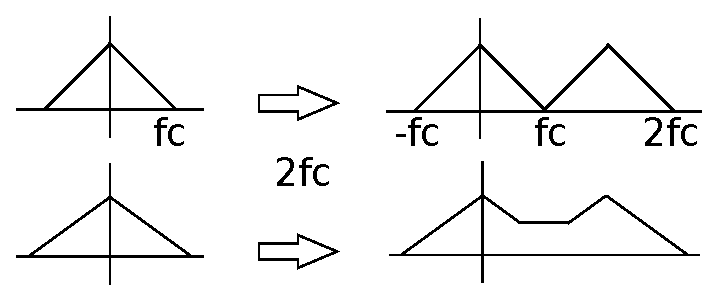
\includegraphics[width=\textwidth]{../images/lec1/FVE_image_2}
\end{figure}

On the figure above, the sampling theorem stated that when the sampling frequency is twice of the maximum frequency ($fs_1=2fc_1$) of the original signal ($fc_1$), then the signal sampled will not be distorted. However, if the same sampling frequency ($fs_1=2fc_1$) is used to sample original signal with maximum frequency, then the sampled signal is distorted because $fs_1 < 2fc_2$. 

\subsection*{Discrete Time Signal Property}
\subparagraph*{Time Shift} $x(t - t_0)$: $x(t)$ shifted $t_0 | t_0>0$ unit toward the right. Under this form, $t_0<0$ shift will be toward the left.
\subparagraph*{Time Reversal/Folding} $x(-t)$ is the same graph as $x(t)$ except it's flipped about the y-axis.
\subparagraph*{Time Scaling} $x(\alpha t)$ will be a new shape based on $x(t)$ where the x co-ordinates correspond to each of the y co-ordinates on the curve $x(t)$ will be divided by $\alpha$. To translate that to math equations:
\begin{align*}
    x_1 = x(t), x_2 = x(\alpha t) \leftrightarrow (\frac{x_1}{\alpha}, y) = (x_2, y)
\end{align*}
Important: When you have a mix of time scaling and shift and reversal, the order of which you follow is \textbf{Shift $\rightarrow$ Flip $\rightarrow$ Scale}.

\subparagraph*{Even \& Odd Signal} Every signal can be broken down into an even and an odd part.
$$x(t) = Ev(x(t)) + Od(x(t))$$
And the part has some uniqueness in it to distinguish one part from the other by looking at the part's time reversal shape.
\begin{align*}
    Ev(x(t))&: x(t) = x(-t) \\
    Od(x(t))&: -x(t) = x(-t)
\end{align*}
In otherwords, to determine if a signal is \textbf{strictly} odd or even, check its time reversal shape and see which statement will fit. If the signal is neither \textbf{strictly} odd or even, then you would need to broke down the signal into $Ev(x(t))$ and $Od(x(t))$ using the equation above.

\subparagraph*{Periodicity} $x(t+T) = x(t)$ means $y_0 = x(t_0)$ can be found again after T seconds for all $t$ in $x$.
